\documentclass[a4paper, 10pt]{article}

\usepackage{vmargin}

\setmarginsrb{2cm}{0cm}{2cm}{0,2cm}{1cm}{1,5cm}{1cm}{1,5cm}
%1 est la marge gauche
%2 est la marge en haut
%3 est la marge droite
%4 est la marge en bas
%5 fixe la hauteur de l'entête
%6 fixe la distance entre l'entête et le texte
%7 fixe la hauteur du pied de page
%8 fixe la distance entre le texte et le pied de page
%------------------------------Packages généraux------------------------------

\usepackage[english]{babel}
\usepackage[T1]{fontenc}
\usepackage{ae}
\usepackage[utf8]{inputenc}
\usepackage{scrextend}
\usepackage{hyperref}

%-------------------------Mathématiques------------------------------
\usepackage{amsmath}
\usepackage{amssymb}
\usepackage{amsthm}
\usepackage{amsfonts}
\usepackage{eucal}
\newcommand\independent{\protect\mathpalette{\protect\independenT}{\perp}}
\def\independenT#1#2{\mathrel{\rlap{$#1#2$}\mkern2mu{#1#2}}}
%-----------------------Codes et algorithmes--------------------------
\usepackage{algorithm}
\usepackage{algorithmic}
\usepackage{clrscode3e}

%------------------------------Graphics------------------------------

\usepackage{graphicx}
\usepackage{fancyhdr}
\usepackage{fancybox}
\usepackage{color}
\usepackage{pgf, tikz}
\usetikzlibrary{arrows, automata}
%\usepackage{slashbox}
%------------------------------Syntaxe------------------------------

\usepackage{listings}
\lstloadlanguages{Matlab}

\def\refmark#1{\hbox{$^{\ref{#1}}$}}
\DeclareSymbolFont{cmmathcal}{OMS}{cmsy}{m}{n} %Mathcal correcte
\DeclareSymbolFontAlphabet{\mathcal}{cmmathcal}

%------------------------------Inclure code MatLab------------------------------

\usepackage{listings}
\newcommand*\styleC{\fontsize{9}{10pt}\usefont{T1}{ptm}{m}{n}\selectfont }
\newcommand*\styleD{\fontsize{9}{10pt}\usefont{OT1}{pag}{m}{n}\selectfont }

%------------------Sub-sections--------%
\usepackage{titlesec}
\usepackage{hyperref}

\renewcommand\thesubsubsection{\alph{subsubsection}}

\titleclass{\subsubsubsection}{straight}[\subsubsection]

\newcounter{subsubsubsection}[subsubsection]
\renewcommand\thesubsubsubsection{\thesubsubsection.\arabic{subsubsubsection}}

\titleformat{\subsubsubsection}
  {\normalfont\normalsize\bfseries}{\thesubsubsubsection}{1em}{}
\titlespacing*{\subsubsubsection}
{0pt}{3.25ex plus 1ex minus .2ex}{1.5ex plus .2ex}


\makeatletter
% on fixe le langage utilisé
\lstset{language=matlab}
\edef\Motscle{emph={\lst@keywords}}
\expandafter\lstset\expandafter{%
  \Motscle}
\makeatother


\definecolor{Ggris}{rgb}{0.45,0.48,0.45}

\lstset{emphstyle=\rmfamily\color{blue}, % les mots réservés de matlab en bleu
basicstyle=\styleC,
keywordstyle=\ttfamily,
commentstyle=\color{Ggris}\styleD, % commentaire en gris
numberstyle=\tiny\color{red},
numbers=left,
numbersep=10pt,
lineskip=0.7pt,
showstringspaces=false}
%  % inclure le fichier source
\newcommand{\FSource}[1]{%
\lstinputlisting[texcl=true]{#1}
}

\usepackage[section]{placeins}

\let\cleardoublepage\clearpage

\usepackage{hyperref}

 \hypersetup{
    colorlinks = true,
    linkcolor=black,
    urlcolor = black
    }
%------------------------------Début du document------------------------------
\begin{document}
%------------------------------Page de garde------------------------------


  % \frontmatter
  %\tableofcontents
   \newpage
   \setcounter{page}{1}
   %%%%%%%%% TP 3 %%%%%%%%%%%
   \section{Games and Adversarial search (25/10/2018)}
   \subsection{Objectives}
    At the end of this repetition you should be able to:
   \begin{itemize}
       \item Define formally the search problem associated to a game (IPATTU\footnote{Initial state - Player function - Actions function - Transition model - Terminal test - Utility function})
       \item Define and apply the Minimax algorithm
       \item Define and apply $\alpha-\beta$ version of Minimax algorithms
       \item Define H-Minimax, Expectiminimax, Monte-Carlo Tree Search
   \end{itemize}
   \subsection{Exercises}
   \subsubsection{Tic Tac Toe ($\approx$ 30 min)}
   "\textit{Tic-tac-toe (also known as noughts and crosses or Xs and Os) is a paper-and-pencil game for two players, X and O, who take turns marking the spaces in a $3\times 3$ grid. The player who succeeds in placing three of their marks in a horizontal, vertical, or diagonal row wins the game.}"\footnote{https://en.wikipedia.org/wiki/Tic-tac-toe} \\
   We define $X_n$ as the number of rows, columns, or diagonals with exactly n X's and no O's. Similarly, $O_n$ is the number of rows, columns, or diagonals
with just n O's. The utility function assigns $+1$ to any position with $X_3 = 1$ and $-1$ to any
position with $O_3 = 1$. All other terminal positions have utility 0. For nonterminal positions,
we use a linear evaluation function defined as $Eval(s) = 3X_2(s)+X_1(s)-(3O_2(s)+O_1(s))$.\\
\begin{enumerate}
    \item Define the search problem associated with the tic tac toe game.
    \item Approximately how many possible games of tic-tac-toe are there?
    \item Show the whole game tree starting from an empty board down to depth 2 (i.e., one X
and one O on the board), taking symmetry into account.
    \item Mark on your tree the evaluations of all the positions at depth 2.
    \item Using the minimax algorithm, mark on your tree the backed-up values for the     positions at depths 1 and 0, and use those values to choose the best starting move.
    \item Circle the nodes at depth 2 that would not be evaluated if alpha–beta pruning were
applied, assuming the nodes are generated in the optimal order for alpha–beta pruning.
\end{enumerate}
\subsubsection{Chess and transposition table ($\approx 15$ min)}
Suppose you have a chess program that can evaluate 16 million nodes per second.
Decide on a compact representation of a game state for storage in a transposition table.
\begin{enumerate}
    \item About how many entries can you fit in a 4-gigabyte in-memory table?
    \item Will that be enough for the three minutes of search allocated for one move?
    \item How many table lookups can you do in the time it would take to do one evaluation? Suppose that you have a 3,2GHz machine and that it takes 20 operations to do one lookup on the transposition table.
    %\item Now suppose the transposition table is stored on disk. About how many evaluations could you do in the time it takes to do one disk seek with standard disk hardware?
\end{enumerate}

   \subsubsection{Quizz ($\approx$ 15 min)}
   \begin{enumerate}
       \item In a fully observable, turn-taking, zero-sum game between two perfectly rational players, it does not help the first player to know what strategy the second player is using that is, what move the second player will make, given the first player’s move.
       \item What is a quiescent position?
       %\item What is the meaning of Q in the formula: $\frac{Q(n', p)}{N(n')} + c\sqrt{\frac{2\log N(n)}{N(n'}}$
       %\item What is the meaning of N in the formula: $\frac{Q(n', p)}{N(n')} + c\sqrt{\frac{2\log N(n)}{N(n'}}$
       \item What is encouraged by each term of the sum in the formula: $\frac{Q(n', p)}{N(n')} + c\sqrt{\frac{2\log N(n)}{N(n'}}$
       \item Which heuristic is correct (see image below)?
   \end{enumerate}
   \begin{figure}[H]
       \centering
       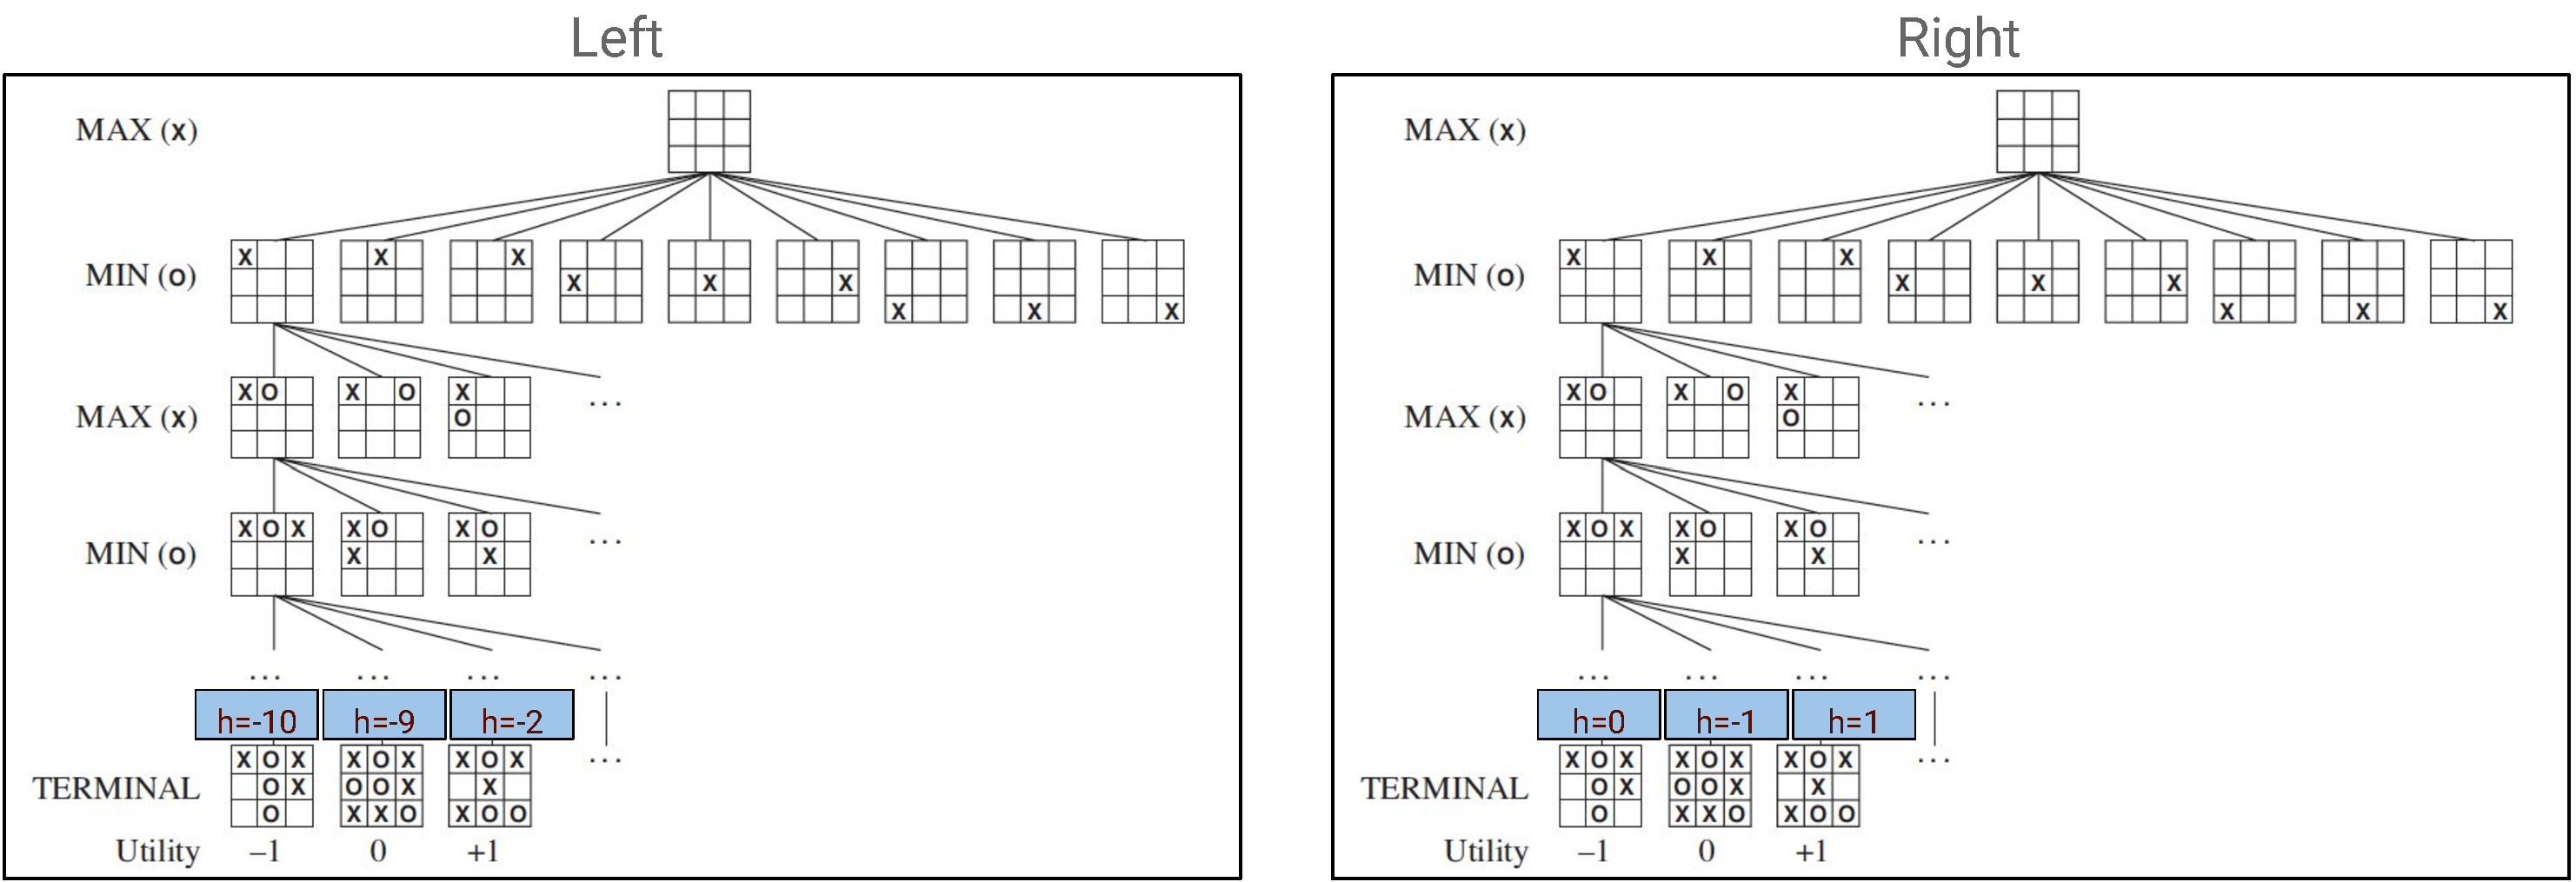
\includegraphics[width=1.\textwidth]{figures/trees.pdf}
       \caption{Two possible heuristics}
       \label{fig:my_label}
   \end{figure}
\end{document}
